\section{Quick prototype}

We implemented our fast technique on top of \textsf{libpolycrypto}~\cite{libpolycrypto}, a library that implements Kate-Zaverucha-Goldberg (KZG)~\cite{KZG10} polynomial commitments together with the Feist-Khovratovich (FK) technique~\cite{FK20} for computing all KZG proofs.
Our code is available at:
\begin{center}
    \url{https://github.com/alinush/fast-pointproofs}
\end{center}

\noindent We ran three benchmarks on a Macbook Pro with a 2.4 GHz 8-Core Intel Core i9 and 32 GB of RAM:
\begin{itemize}
    \item Our fast $O(N\log{N})$ time proof precomputation for Pointproofs from \cref{s:pointproofs:precompute-all-proofs}
    \item The naive $O(N^2)$ time proof precomputation for Pointproofs
    \item The fast $O(N\log{N})$ time proof precomputation for~\cite{TAB+20}.
\end{itemize}

\noindent We summarize the results in \cref{f:benchmarks}.
\begin{figure}[h]
    \centering
    \textbf{Precomputing all $N$ proofs in Pointproofs and in ~\cite{TAB+20}}\par\medskip
    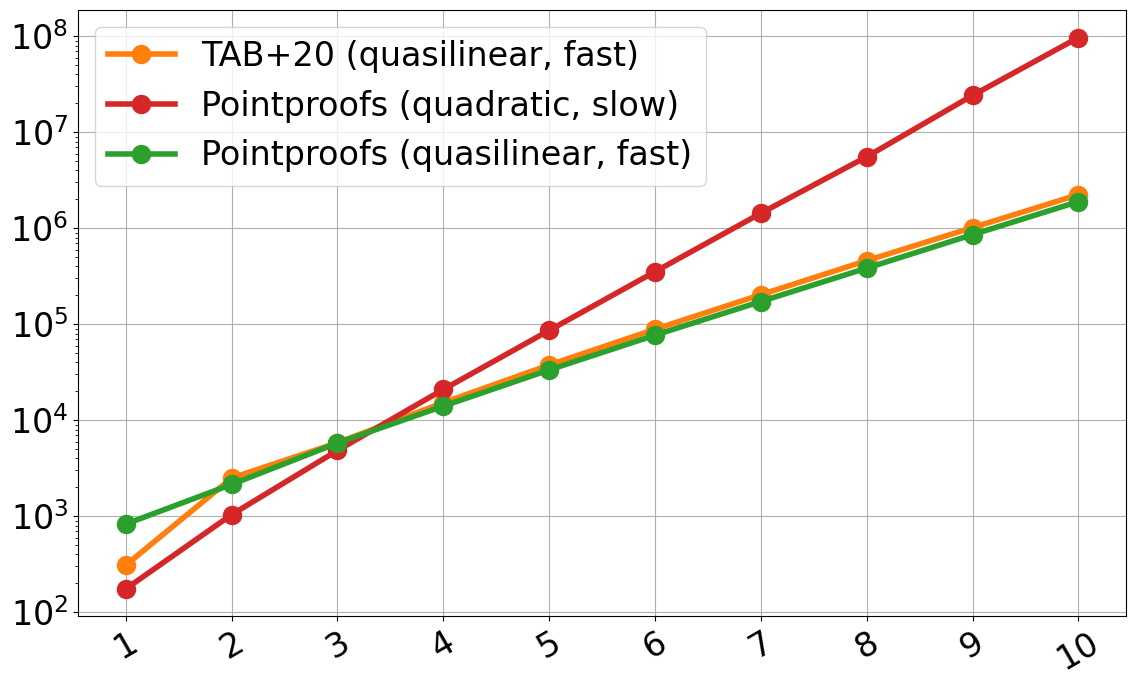
\includegraphics[width=0.80\columnwidth]{fk-vs-pointproofs.png}
    \caption{
        The $x$-axis is $\log_2{N}$, where $N$ is the size of the vector of messages $\vect{m}$.
        The $y$-axis is the number of microseconds it took to compute all $N$ proofs for the specified scheme.
        Clearly, our faster $O(N\log{N})$ algorithm for computing all $N$ proofs in Pointproofs scales much better than the naive $O(N^2)$ one.
        It also performs slightly better than the FK technique used in~\cite{TAB+20}.
    }
    \label{f:benchmarks}
\end{figure}
